\subsection{Experiment}
Since counterbalancing has been applied no interaction effects were expected. In figure ~\ref{fig:efficient_actions} - ~\ref{fig:orientation_changes} this appears indeed to be the case. The Wilcoxon signed-rank tests were therefor performed over the combined data.

\subsubsection{Efficient actions}

A strong and significant main effect of the interaction device was found on the \textsc{efficient actions} $(Z(1) = -3.516, p = .000438, r = .622)$. The medians for the keyboard and leap modes were 1.0 and .228 respectively. See figure~\ref{fig:efficient_actions}.

\begin{figure}[H]
\centering
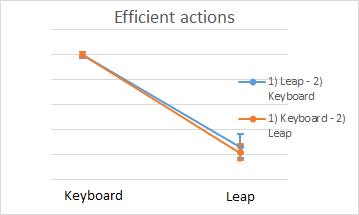
\includegraphics[width=0.5\textwidth]{imgs/results/efficient_actions}
\caption{Efficient actions - the mean and the 95\% intervals are plotted for both modes. The plots was split on the order of the interaction device. There is only a main effect of interaction device and no interaction device x order interaction effect.}
\label{fig:efficient_actions}
\end{figure}

\subsubsection{Average Time}

A strong and significant main effect of the interaction device was found on the \textsc{average time} $(Z(1) = -3.516, p = .000438, r = .622)$. The medians for the keyboard and leap modes were 8880 and 246428 respectively. See figure~\ref{fig:average_time}.

\begin{figure}[H]
\centering
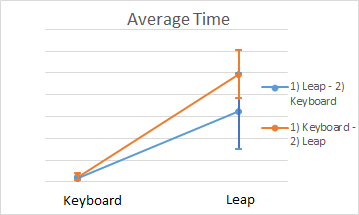
\includegraphics[width=0.5\textwidth]{imgs/results/average_time}
\caption{Average Time - the mean and the 95\% intervals are plotted for both modes. The plots was split on the order of the interaction device. There is only a main effect of interaction device and no interaction device x order interaction effect.}
\label{fig:average_time}
\end{figure}

\subsubsection{Block Repositioning}

A strong and significant main effect of the interaction device was found on the \textsc{block repositioning} $(Z(1) = -3.414, p = .000640, r = .604)$. The medians for the keyboard and leap modes were 0 and 16 respectively. See figure~\ref{fig:block_repositioning}.

\begin{figure}[H]
\centering
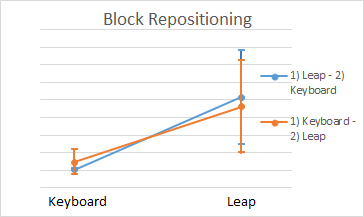
\includegraphics[width=0.5\textwidth]{imgs/results/block_repositioning}
\caption{Block Repositioning - the mean and the 95\% intervals are plotted for both modes. The plots was split on the order of the interaction device. There is only a main effect of interaction device and no interaction device x order interaction effect.}
\label{fig:block_repositioning}
\end{figure}

\subsubsection{Orientation Changes}

A strong and significant main effect of the interaction device was found on the \textsc{orientation changes} $(Z(1) = -3.297, p = .000979, r = .583)$. The medians for the keyboard and leap modes were 0 and 35 respectively. See figure~\ref{fig:orientation_changes}.

\begin{figure}[H]
\centering
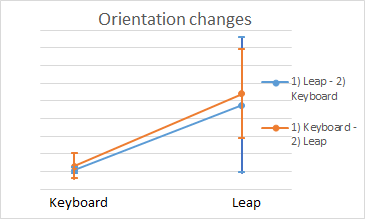
\includegraphics[width=0.5\textwidth]{imgs/results/orientation_changes}
\caption{Orientation Changes - the mean and the 95\% intervals are plotted for both modes. The plots was split on the order of the interaction device. There is only a main effect of interaction device and no interaction device x order interaction effect.}
\label{fig:orientation_changes}
\end{figure}



